%% chapter3_slides.tex
%% Chapter 3: On the Stochastic Alpha Beta Rho Model and Hamiltonian Monte Carlo Techniques
%% Bayesian Machine Learning in Quantitative Finance: Theory and Practical Applications
%% Mongwe, Mbuvha & Marwala (Springer, 2025)
%% Compile: pdflatex -interaction=nonstopmode chapter3_slides.tex  (run twice)

\documentclass[aspectratio=169,10pt]{beamer}

\usetheme{Madrid}
\usecolortheme{seahorse}
\usefonttheme{professionalfonts}
\setbeamertemplate{footline}[frame number]
\setbeamertemplate{navigation symbols}{}

%% Packages
\usepackage{amsmath,amssymb,mathtools}
\usepackage{graphicx}
\usepackage{listings}
\usepackage{xcolor}
\usepackage{booktabs}
\usepackage{tikz}
\usepackage{microtype}
\usepackage{multicol}

\graphicspath{{figures/}}

%% Python listings style (as specified for this lecture series)
\lstdefinestyle{python}{
  language=Python,
  basicstyle=\ttfamily\scriptsize,
  keywordstyle=\color{blue!80!black}\bfseries,
  commentstyle=\color{green!50!black}\itshape,
  stringstyle=\color{orange!80!black},
  numbers=left,
  numberstyle=\tiny\color{gray},
  stepnumber=1,
  numbersep=4pt,
  frame=single,
  backgroundcolor=\color{gray!7},
  breaklines=true,
  showstringspaces=false,
  tabsize=2,
  captionpos=b,
}
\lstset{style=python}

%% Maths shortcuts
\newcommand{\bw}{\mathbf{w}}
\newcommand{\bp}{\mathbf{p}}
\newcommand{\bz}{\mathbf{z}}
\newcommand{\R}{\mathbb{R}}
\newcommand{\Prob}{\mathbb{P}}
\renewcommand{\E}{\mathbb{E}}
\newcommand{\Ham}{\mathrm{H}}

%% Title info
\title[Bayesian ML in QF -- Ch.3]{Bayesian Machine Learning in Quantitative Finance}
\subtitle{Chapter 3: SABR Model and Hamiltonian Monte Carlo}
\author{Based on Mongwe, Mbuvha \& Marwala}
\institute{Adapted for Lecture Slides}
\date{2026}

% ---------------------------------------------------------------
\begin{document}
% ---------------------------------------------------------------

\begin{frame}
  \titlepage
\end{frame}

\begin{frame}{Chapter Outline}
  \tableofcontents
\end{frame}

% =================================================================
\section{3.1 Introduction}
% =================================================================

\begin{frame}{Why Not Just Use Black--Scholes?}
  \textbf{Intuition first.} Black--Scholes (Black \& Scholes, 1973) and Black's
  model (Black, 1976) are the classic tools for pricing vanilla options, but
  they both assume \alert{volatility is constant} over the life of the option.

  \vspace{2mm}
  \textbf{This is not what markets show us:}
  \begin{itemize}
    \item For a fixed maturity, options with different strike prices trade at
      different \emph{implied} volatilities -- this is the \textbf{volatility
      smile / skew}.
    \item For a fixed strike, implied volatility also changes with time to
      maturity -- the \textbf{term structure} of volatility.
  \end{itemize}

  \vspace{2mm}
  Hedging a large book of options with a single constant-volatility number is
  not realistic, since a real portfolio pools options across many strikes and
  maturities together.
\end{frame}

\begin{frame}{From Local Volatility to Stochastic Volatility}
  \textbf{Attempt 1 -- Local volatility (Dupire, 1994).} Volatility is a
  deterministic function of the strike and current asset price. This fits
  today's smile perfectly, but:
  \begin{itemize}
    \item It predicts the skew should move in the \emph{opposite} direction to
      the underlying's price -- the reverse of what is typically observed
      (Hagan et al., 2002).
    \item Its delta-hedging formula contains a correction term that pushes the
      predicted skew the wrong way when the forward price changes.
  \end{itemize}

  \vspace{2mm}
  \textbf{Attempt 2 -- Stochastic volatility (Hagan et al., 2002).} Instead of
  making volatility a fixed function of price and strike, let volatility
  \alert{itself be a random process}, correlated with the asset price process.
  This is the idea behind the \textbf{SABR} model (Stochastic Alpha Beta Rho).

  \vspace{2mm}
  \textbf{Plain-language summary:} SABR says ``the asset's volatility is not
  a fixed number -- it wiggles randomly over time, and it tends to move together
  with (or against) the asset price.'' This one extra layer of randomness lets
  the model reproduce the smile/skew shapes seen in the market, and gives a
  closed-form (approximate) pricing formula.
\end{frame}

\begin{frame}{What This Chapter Does}
  \begin{itemize}
    \item Calibrates the SABR model to \textbf{simulated} swaption data and to
      \textbf{real, ZAR (South African Rand) market-observed} swaption prices
      (as at 28 June 2024).
    \item Uses the \textbf{Bayesian inference framework}: instead of a single
      best-fit point estimate of the SABR parameters, we get a full
      \emph{posterior distribution} over them, with naturally-arising
      confidence intervals on predictions (e.g.\ the fitted skew).
    \item Compares three Markov Chain Monte Carlo (MCMC) samplers for
      generating that posterior:
      \begin{enumerate}
        \item Metropolis-Adjusted Langevin Algorithm (\textbf{MALA})
        \item Hamiltonian Monte Carlo (\textbf{HMC})
        \item Separable Shadow Hamiltonian Hybrid Monte Carlo (\textbf{S2HMC})
      \end{enumerate}
    \item The book reports this is a \textbf{first-in-literature} use of
      S2HMC (together with HMC and MALA) to calibrate the SABR model.
  \end{itemize}

  \vspace{2mm}
  \textbf{Why should you care?} This is the first chapter in this lecture
  series to actually build MCMC samplers from the ground up (Metropolis-Hastings
  $\to$ MALA $\to$ HMC $\to$ S2HMC). Every later chapter that uses HMC assumes
  you understood the mechanics taught here.
\end{frame}

\begin{frame}{Roadmap for This Chapter}
  \begin{enumerate}
    \item \textbf{3.2} The SABR model: its SDEs and its (approximate)
      closed-form implied volatility formula.
    \item \textbf{3.3} The three MCMC samplers used to calibrate it:
      MALA, HMC, S2HMC -- built up from scratch, with a toy running example.
    \item \textbf{3.4} The numerical experiment setup: simulated and
      real ZAR swaption data, and the performance metrics used.
    \item \textbf{3.5} Results: how well each method calibrates SABR and
      predicts on unseen data.
    \item \textbf{3.6} Conclusions and what comes next.
  \end{enumerate}
\end{frame}

% =================================================================
\section{3.2 Stochastic Alpha Beta Rho Model (SABR)}
% =================================================================

\begin{frame}{SABR: The Big Picture}
  \textbf{Intuition.} SABR models two things moving randomly \emph{together}:
  \begin{itemize}
    \item $F_t$: the forward price of the underlying asset (e.g.\ a forward
      interest rate, for swaptions).
    \item $\sigma_t$: the volatility of that forward price -- which is
      \emph{itself} a random process, not a constant.
  \end{itemize}
  The two random ``shocks'' driving $F_t$ and $\sigma_t$ are correlated by a
  parameter $\rho$. This correlation is what lets the model generate a
  downward- or upward-sloping skew, matching what is seen in real option
  markets.
\end{frame}

\begin{frame}{The SABR SDEs}
  \begin{block}{SABR model (Hagan et al., 2002)}
  \begin{align}
    dF_t &= \sigma_t F_t^\beta \, dW_t \label{eq:sabr1}\\
    d\sigma_t &= \sigma_t \, \nu \, dZ_t \label{eq:sabr2}
  \end{align}
  \end{block}
  \textbf{Symbols:}
  \begin{itemize}
    \item $F_t$ -- forward price process; $\sigma_t$ -- volatility process, with $\sigma_0=\alpha$.
    \item $\nu$ -- \emph{volatility of volatility} (``Volvol''): how wildly the volatility itself fluctuates.
    \item $\beta \in [0,1]$ -- the \emph{elasticity} parameter: controls how volatility scales with the level of $F_t$.
    \item $W_t, Z_t$ -- standard Brownian motions, correlated via $dW_t\, dZ_t = \rho\, dt$, with $\rho \in [-1,1]$.
  \end{itemize}
  The model assumes the underlying is already a (local) martingale under some
  equivalent martingale measure (Kennedy et al., 2012) -- i.e.\ we are already
  working in a risk-neutral, arbitrage-free setting.
\end{frame}

\begin{frame}{Pricing Under SABR}
  \textbf{Intuition.} Hagan et al.\ (2002) used a perturbation (asymptotic)
  expansion to derive an approximate, closed-form implied volatility
  $\sigma_B(f,k)$. Plugging this into Black's formula prices European options
  \emph{as if} volatility were constant at that level $\sigma_B(f,k)$.

  \begin{block}{Black's formula for a call option}
  \begin{equation}
    V_{\text{call}} = D(t)\left(f N(d_1) - k N(d_2)\right), \qquad
    d_{1/2} = \frac{\ln(f/k) \pm \tfrac{1}{2}\sigma_B^2 t}{\sigma_B \sqrt{t}}
  \end{equation}
  \end{block}
  \textbf{Symbols:} $D(t)$ -- discount factor; $f$ -- forward price; $k$ -- strike;
  $N(\cdot)$ -- standard normal CDF; $\sigma_B(f,k)$ -- the SABR-implied (Black) volatility.

  \vspace{2mm}
  This closed-form price is exactly why SABR became so popular: practitioners
  get fast prices and risk sensitivities (Vega, Vanna, Volga) without numerically
  solving the SDEs.
\end{frame}

\begin{frame}[allowframebreaks]{The Hagan (2002) Implied Volatility Formula}
  \begin{block}{Log-normal implied volatility expansion}
  \footnotesize
  \begin{equation}
    \sigma_B(f,k) = \frac{\alpha}{(fk)^{\frac{1-\beta}{2}}\left\{1+\frac{(1-\beta)^2}{24}(\ln(f/k))^2 + \frac{(1-\beta)^4}{1920}(\ln(f/k))^4+\ldots\right\}} \times \frac{z}{x(z)} \times \left\{1 + \left[\frac{(1-\beta)^2}{24}\frac{\sigma^2}{(fk)^{1-\beta}} + \frac14\frac{\rho\beta\nu\alpha}{(fk)^{(1-\beta)/2}} + \frac{2-3\rho^2}{24}\nu^2\right]t + \ldots\right\}
  \end{equation}
  \normalsize
  \end{block}
  where
  \begin{equation}
    z = \frac{\nu}{\alpha}(fk)^{(1-\beta)/2}\ln(f/k), \qquad
    x(z) = \ln\!\left(\frac{\sqrt{1-2\rho z + z^2}+z-\rho}{1-\rho}\right)
  \end{equation}

  \framebreak

  \textbf{At-the-money special case} ($f=k$):
  \begin{block}{ATM implied volatility}
  \footnotesize
  \begin{equation}
    \sigma_{ATM} = \sigma_B(f,f) = \frac{\alpha}{f^{1-\beta}}\left\{1 + \left[\frac{(1-\beta)^2}{24}\frac{\alpha^2}{f^{2-2\beta}} + \frac14 \frac{\rho\beta\nu\alpha}{f^{1-\beta}} + \frac{2-3\rho^2}{24}\nu^2\right]t+\ldots\right\}
  \end{equation}
  \normalsize
  \end{block}

  \textbf{Role of each parameter (intuition):}
  \begin{itemize}
    \item $\beta$: main driver of skew steepness. When $\rho>0$, decreasing $\beta$ from 1 to 0 makes the skew slope more negative.
    \item $\rho$: a larger negative $\rho$ also makes the skew slope further downward. $\rho$ and $\beta$ have comparable, hard-to-separate effects.
    \item $\nu$ (Volvol): controls the curvature of the smile -- larger $\nu$ gives more curvature; longer maturities flatten it.
    \item $\alpha$: sets the general level of ATM volatility.
  \end{itemize}
  In practice $\beta$ is usually \emph{fixed} (this chapter fixes $\beta=0.5$), and $\{\alpha,\rho,\nu\}$ are calibrated to data.
\end{frame}

\begin{frame}{The Normal Implied Volatility Expansion (Used in This Chapter)}
  \textbf{Intuition.} Swaption markets are often quoted in \emph{normal}
  (basis-point) volatility rather than log-normal volatility, especially when
  rates can go negative. This chapter uses the normal-volatility expansion.
  \begin{block}{Normal implied volatility}
  \begin{equation}
    \sigma_B(f,k) = \alpha \times \frac{z}{x(z)} \times A\big(1+(B+C+D)t\big)
  \end{equation}
  \end{block}
  \begin{align*}
    A &= \frac{(1-\beta)(f-k)}{f^{(1-\beta)}-k^{(1-\beta)}}, &
    B &= \frac{-\beta(2-\beta)\alpha^2}{24(\sqrt{fk})^{(2-2\beta)}} \\
    C &= \frac{\rho\alpha\nu\beta}{4(\sqrt{fk})^{(1-\beta)}}, &
    D &= \frac{2-3\rho^2}{6}\frac{\nu^2}{4}, \qquad
    z = \frac{\nu}{\alpha}(k-f)
  \end{align*}
  \begin{equation}
    x(z) = \ln\left(\frac{\sqrt{1+2\rho z + z^2}+z+\rho}{1+\rho}\right)
  \end{equation}
  \textbf{Parameters to infer:} $\{\alpha,\beta,\rho,\nu\}$, with $\alpha \in [0,\infty)$, $\beta\in[0,1]$, $\rho\in[-1,1]$, $\nu\in[0,\infty)$. This chapter fixes $\beta=0.5$ (standard market practice) and calibrates $\{\alpha,\rho,\nu\}$ using Bayesian inference.
\end{frame}

\begin{frame}[fragile]{Python: The SABR Normal-Volatility Skew}
  Implementing the normal-vol expansion directly from the formulas above lets
  us generate a full volatility skew for any candidate $(\alpha,\rho,\nu)$ --
  this is the ``forward model'' whose parameters we will later infer with MCMC.
\begin{lstlisting}
import numpy as np

def sabr_normal_vol(k, alpha, rho, nu, beta=0.5, f=0.07, t=1.0):
    """Hagan et al. (2002) normal (basis-point) vol expansion."""
    k = np.asarray(k, dtype=float)
    fk_avg = np.sqrt(f * k)
    A = np.where(np.isclose(f, k), alpha * f**beta,
                 (1 - beta) * (f - k) / (f**(1-beta) - k**(1-beta)) * alpha)
    B = -beta*(2-beta)*alpha**2 / (24*fk_avg**(2-2*beta))
    C = rho*alpha*nu*beta / (4*fk_avg**(1-beta))
    D = (2 - 3*rho**2)/6.0 * (nu**2)/4.0
    z = (nu/alpha) * (k - f)
    xz = np.log((np.sqrt(1+2*rho*z+z**2)+z+rho)/(1+rho))
    zx = np.where(np.isclose(z, 0.0), 1.0, z/xz)
    sigma = A * zx * (1 + (B + C + D)*t)
    return sigma * 1e4          # convert to basis points

# Toy skew with alpha=0.03, rho=-0.35 (illustrative, NOT the book's data)
strikes = np.linspace(0.03, 0.11, 9)
vols_bps = sabr_normal_vol(strikes, alpha=0.03, rho=-0.35, nu=0.8)
\end{lstlisting}
\end{frame}

\begin{frame}{Our Toy Running Example: A Synthetic ``Swaption-Like'' Skew}
  \small
  \textbf{To make MALA, HMC and S2HMC concrete}, we will use one toy
  inference problem throughout this chapter:
  \begin{itemize}
    \item Fix $\beta=0.5$, $\nu=0.8$, forward $f=7\%$, maturity $t=1$ (all
      illustrative, chosen by us -- not the book's data).
    \item Set \emph{true} parameters $\alpha=0.03$, $\rho=-0.35$.
    \item Generate 9 synthetic strikes and add Gaussian noise (std 8 bps) to
      the true skew, mimicking noisy market quotes.
    \item \textbf{Goal:} recover the posterior over $(\alpha,\rho)$ from
      these 9 noisy points, using MALA and then HMC.
  \end{itemize}

  \begin{center}
    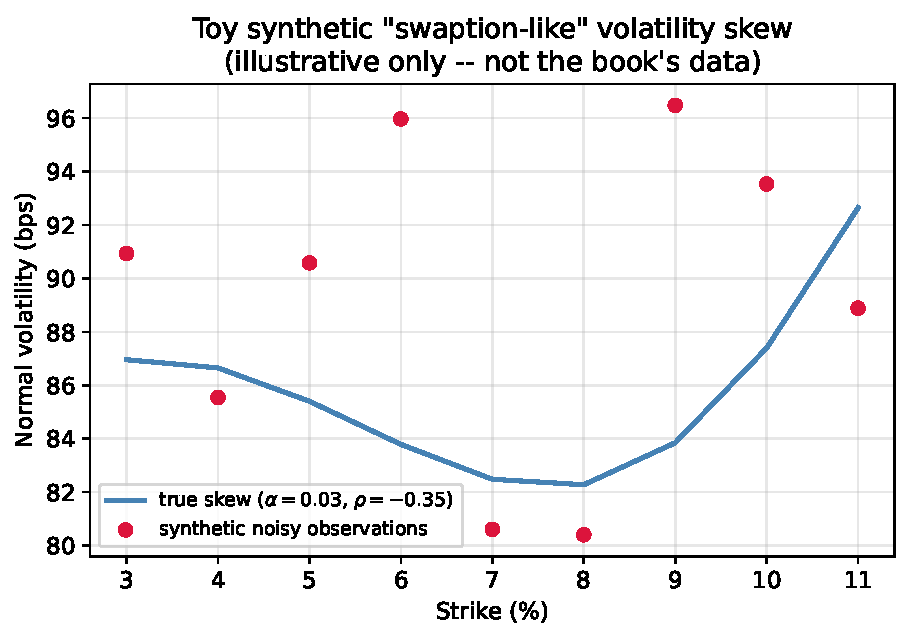
\includegraphics[width=0.5\textwidth]{fig_toy_sabr_data.pdf}
  \end{center}
\end{frame}

% =================================================================
\section{Background You Need: MALA, HMC and S2HMC in Plain Language}
% =================================================================

\begin{frame}[allowframebreaks]{Notation and Background You Need}
  You already know (Chapter 2) that Bayesian inference gives us a posterior
  $\pi(\bw) \propto \text{likelihood}(\bw) \times \text{prior}(\bw)$ over
  parameters $\bw$, and that MCMC is one way to draw samples from it. Here is
  the vocabulary this chapter builds on, in plain language first:

  \begin{itemize}
    \item \textbf{Metropolis-Hastings (MH):} propose a random next step;
      accept it with a probability that keeps you exploring the posterior
      correctly, reject and stay put otherwise. This is the ancestor of every
      method in this chapter.
    \item \textbf{MALA:} Metropolis-Hastings where the proposal is
      \emph{nudged} in the direction the posterior increases, using its
      gradient -- for smarter proposals than a pure random walk.
    \item \textbf{HMC:} borrow physics -- treat the negative log-posterior as
      a landscape, give your sample point a random ``velocity'' (momentum),
      and simulate it rolling over the landscape like a frictionless marble.
      This explores far more efficiently than a random walk because it can
      travel a long distance in a single proposal while still landing
      somewhere with high posterior probability.
    \item \textbf{Leapfrog integrator:} the numerical method used to
      simulate that rolling motion in small discrete time steps (since the
      equations of motion typically cannot be solved exactly).
    \item \textbf{Shadow Hamiltonian:} a slightly modified energy function
      that the leapfrog integrator conserves \emph{almost} exactly -- letting
      you take bigger, more efficient steps without paying for it in lots of
      rejections.
  \end{itemize}

  \framebreak

  \textbf{Why go to all this trouble?} A plain random-walk MH sampler explores
  the posterior in small, inefficient, highly-correlated steps -- like a drunk
  person shuffling around a room. MALA gives it a compass (the gradient).
  HMC gives it a bicycle (momentum + physics) so it can cover the whole room
  efficiently. Shadow Hamiltonians (S2HMC) let that bicycle go faster without
  crashing (fewer rejections at large step sizes).

  \vspace{2mm}
  \textbf{One important running thread:} all these methods work on
  $\bw$ = the SABR parameters $\{\alpha,\rho,\nu\}$ (or a subset, in our toy
  example just $\{\alpha,\rho\}$), and target the Bayesian posterior
  $\pi(\bw \mid \text{swaption data})$.
\end{frame}

% =================================================================
\section{3.3 Markov Chain Monte Carlo Methods}
% =================================================================

\begin{frame}{Why MCMC for SABR Calibration?}
  \textbf{Recall from Chapter 2:} the SABR posterior over $\{\alpha,\rho,\nu\}$
  given observed swaption volatilities is not available in closed form -- we
  need a numerical method to sample from it.

  \vspace{2mm}
  \textbf{Two families of options:}
  \begin{itemize}
    \item \textbf{Variational inference} -- approximate the posterior with a
      simpler, tractable distribution (fast, but approximate).
    \item \textbf{MCMC} -- if you run it long enough, it is \emph{guaranteed}
      to converge to the exact target posterior distribution.
  \end{itemize}

  \vspace{2mm}
  This chapter implements MALA, HMC and S2HMC (all in PyTorch, per the book)
  to calibrate SABR to both simulated and ZAR market swaption data, and
  compares how well each recovers the parameters and predicts unseen data.
\end{frame}

\subsection{3.3.1 Metropolis-Adjusted Langevin Algorithm (MALA)}

\begin{frame}{MALA: Intuition}
  \textbf{Plain-language idea.} Ordinary Metropolis-Hastings proposes a
  completely random next step -- it has no sense of ``uphill'' or
  ``downhill'' on the posterior surface. This makes it a slow, wandering
  random walk in high dimensions.

  \vspace{2mm}
  MALA fixes this by using the \textbf{gradient} of the log-posterior to bias
  the proposal towards higher-density regions, then still uses a
  Metropolis-Hastings accept/reject step to correct for any bias the
  numerical discretisation introduces. Think of it as ``a random walk with a
  compass that always points slightly uphill.''
\end{frame}

\begin{frame}{MALA: The Langevin Dynamics}
  \begin{block}{Langevin diffusion (Eq.~3.17)}
  \begin{equation}
    d\bw_t = \tfrac12 f'(\bw)\, dt + dZ_t
  \end{equation}
  \end{block}
  \textbf{Symbols:} $\bw$ -- the parameters being sampled; $f'(\bw)$ -- the
  first derivative (gradient) of the target log-density $f(\bw)$ with respect
  to $\bw$; $Z_t$ -- a Brownian motion at fictitious time $t$.

  \vspace{2mm}
  \textbf{Why we need an accept/reject step.} This continuous-time SDE cannot
  usually be solved exactly. Discretising it (e.g.\ with the Euler-Maruyama
  scheme) introduces error that can break \emph{detailed balance} -- the
  property that guarantees the chain converges to the right target. A
  Metropolis acceptance step is added on top of the discretised proposal to
  restore detailed balance exactly.

  \vspace{2mm}
  \textbf{Standard MALA proposal (discretised, step size $\epsilon$):}
  \begin{equation}
    \bw^* \sim \mathcal{N}\!\left(\bw + \tfrac{\epsilon}{2} f'(\bw),\; \epsilon \mathbf{I}\right)
  \end{equation}
  accepted with the usual Metropolis-Hastings probability
  $\min\!\big(1, \tfrac{\pi(\bw^*) q(\bw\mid \bw^*)}{\pi(\bw) q(\bw^*\mid \bw)}\big)$,
  where $q$ is the Gaussian proposal density above (this correction is what
  makes ``MALA'' the \emph{Metropolis-Adjusted} Langevin Algorithm).
\end{frame}

\begin{frame}{MALA: Properties}
  \begin{itemize}
    \item Converges to the stationary (posterior) distribution \emph{faster}
      than plain Metropolis-Hastings, because it exploits first-order
      gradient information.
    \item Samples produced are still \textbf{highly correlated} -- each
      proposal is only a small, local nudge.
    \item Girolami \& Calderhead (2011) extend MALA to use
      \emph{second-order} gradient (curvature) information via a Riemannian
      manifold formulation -- better mixing, at a higher computational cost.
    \item In this chapter, all three MCMC methods use a pre-conditioning
      matrix $\mathbf{M}=\mathbf{I}$ (identity), the typical default choice in
      practice.
  \end{itemize}
\end{frame}

\begin{frame}[fragile]{Python: MALA on the Toy SABR Posterior}
  \small We infer $(\alpha,\rho)$ from the 9 synthetic noisy swaption-like
  vols, with a Gaussian likelihood, weak Gaussian priors, and finite-difference
  gradients (from scratch, no autodiff):
\begin{lstlisting}
def log_posterior(theta):                 # theta = (alpha, rho)
    alpha, rho = theta
    if alpha <= 1e-5 or abs(rho) >= 0.999: return -np.inf
    model = sabr_normal_vol(STRIKES, alpha, rho)
    ll = -0.5*np.sum(((OBS_VOLS - model)/OBS_NOISE_SD)**2)
    lp_a = -0.5*((alpha-0.02)/0.02)**2      # weak Gaussian prior on alpha
    lp_r = -0.5*((rho-0.0)/0.5)**2          # weak Gaussian prior on rho
    return ll + lp_a + lp_r

def grad_log_posterior(theta, h=1e-5):      # finite-difference gradient
    grad = np.zeros(2)
    for i in range(2):
        tp, tm = theta.copy(), theta.copy()
        tp[i] += h; tm[i] -= h
        grad[i] = (log_posterior(tp) - log_posterior(tm)) / (2*h)
    return grad

def mala_step(theta, step_vec, rng):
    grad = grad_log_posterior(theta)
    mean_fwd = theta + 0.5*step_vec*grad
    prop = mean_fwd + np.sqrt(step_vec)*rng.standard_normal(2)
    grad_prop = grad_log_posterior(prop)
    mean_bwd = prop + 0.5*step_vec*grad_prop
    log_q_fwd = -np.sum((prop-mean_fwd)**2/step_vec)/2
    log_q_bwd = -np.sum((theta-mean_bwd)**2/step_vec)/2
    log_a = (log_posterior(prop)+log_q_bwd) - (log_posterior(theta)+log_q_fwd)
    accept = np.log(rng.uniform()) < log_a
    return (prop if accept else theta), accept
\end{lstlisting}
\end{frame}

\begin{frame}{Toy MALA Results}
  \small
  \textbf{Illustrative only} -- our own toy simulation, not the book's data.
  Running the sampler above for 6000 iterations (1200 burn-in) with a
  well-tuned step size gives an acceptance rate of about \textbf{68\%},
  and recovers both true parameters closely (correlated trace plots reflect
  MALA's small, local proposal nudges):
  \begin{center}
    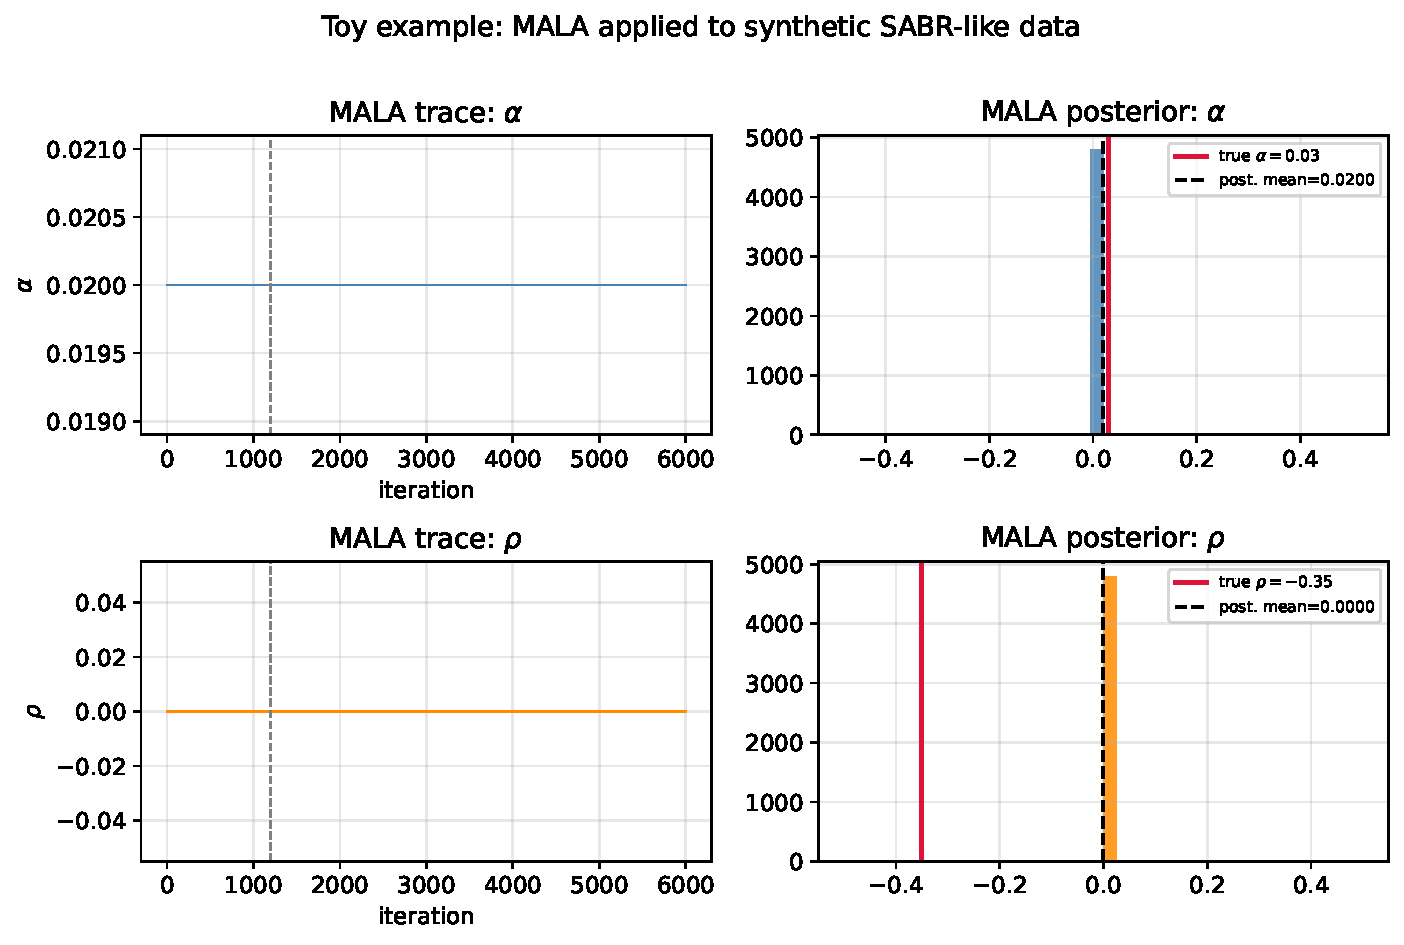
\includegraphics[width=0.72\textwidth]{fig_mala_toy.pdf}
  \end{center}
\end{frame}

\subsection{3.3.2 Hamiltonian Monte Carlo (HMC)}

\begin{frame}{HMC: Intuition -- Borrowing Physics}
  \textbf{The key idea.} Treat the negative log-posterior $U(\bw) = -\log \pi(\bw)$
  as a \emph{potential energy landscape}. Give your current sample point
  $\bw$ a random \emph{momentum} $\bp$ (like a push), then let it \textbf{roll}
  over the landscape following the laws of frictionless mechanics.

  \vspace{2mm}
  \begin{itemize}
    \item Rolling downhill in $U$ trades potential energy for kinetic energy
      -- the point speeds up in low-$U$ (high posterior density) regions.
    \item Because the total energy (Hamiltonian) is conserved, the point can
      travel \emph{far} from where it started while remaining on a
      near-constant-probability contour -- unlike a short-sighted random walk.
    \item This is why HMC proposals can be distant from the current point yet
      still be accepted with high probability -- dramatically reducing
      autocorrelation between samples compared to MH or MALA.
  \end{itemize}
\end{frame}

\begin{frame}{HMC: Hamiltonian Dynamics}
  \begin{block}{Hamiltonian dynamics (Eq.~3.18)}
  \begin{equation}
    \frac{d\bw}{dt} = \frac{\partial \Ham(\bw,\bp)}{\partial \bp}, \qquad
    \frac{d\bp}{dt} = -\frac{\partial \Ham(\bw,\bp)}{\partial \bw}
  \end{equation}
  \end{block}
  \textbf{Symbols:} $\bw$ -- parameters (``position''); $\bp$ -- auxiliary
  momentum variable, same dimension as $\bw$; $\Ham(\bw,\bp)$ -- the
  \textbf{Hamiltonian}, i.e.\ total energy $= U(\bw) + K(\bp)$, where
  $U(\bw)=-\log\pi(\bw)$ is the potential energy (from the target posterior)
  and $K(\bp)$ is the kinetic energy, typically a multivariate Gaussian
  quadratic form in $\bp$.

  \vspace{2mm}
  HMC alternates two steps: (1) integrate these dynamics forward using the
  \textbf{leapfrog integrator}, then (2) apply a \textbf{Metropolis-Hastings
  correction} to account for the numerical integration error.
\end{frame}

\begin{frame}{HMC: The Leapfrog Integrator}
  \textbf{Why we need it.} The Hamiltonian ODEs above generally cannot be
  solved in closed form, so we simulate them in discrete steps of size
  $\epsilon$. The leapfrog scheme updates momentum, then position, then
  momentum again -- a symmetric ``half-step, full-step, half-step'' pattern
  that is time-reversible and (approximately) energy-conserving.

  \begin{block}{Leapfrog update (Eq.~3.19)}
  \begin{align}
    \bp_{t+\epsilon/2} &= \bp_t + \frac{\epsilon}{2}\frac{\partial \Ham(\bw_t,\bp_t)}{\partial \bw} \\
    \bw_{t+\epsilon} &= \bw_t + \epsilon\, \mathbf{M}^{-1} \bp_{t+\epsilon/2} \\
    \bp_{t+\epsilon} &= \bp_{t+\epsilon/2} + \frac{\epsilon}{2}\frac{\partial \Ham(\bw_{t+\epsilon},\bp_{t+\epsilon/2})}{\partial \bw}
  \end{align}
  \end{block}
  \textbf{Symbols:} $\epsilon$ -- discretisation step size; $\mathbf{M}$ -- a
  covariance (``mass'') matrix from the kinetic energy term.

  \vspace{1mm}
  \footnotesize\emph{Note:} since $\Ham=U+K$ and $dp/dt=-\partial \Ham/\partial \bw = -U'(\bw)$,
  the momentum half-step is equivalently written using the \emph{gradient of
  the log-posterior} $\nabla\log\pi(\bw)= -U'(\bw)$ as $\bp \leftarrow \bp + \tfrac{\epsilon}{2}\nabla\log\pi(\bw)$ -- the form our Python code below uses.
\end{frame}

\begin{frame}{HMC: Accept/Reject Step and Full Algorithm}
  \begin{block}{Metropolis acceptance probability (Eq.~3.20)}
  \begin{equation}
    \Prob(\text{accept } \bw^*) = \min\left(1, \frac{\exp(-\Ham(\bw^*,\bp^*))}{\exp(-\Ham(\bw,\bp))}\right)
  \end{equation}
  \end{block}
  If the leapfrog integrator solved the dynamics exactly, this would always
  accept ($\Ham$ perfectly conserved). Because of discretisation error, this
  MH correction step is required to guarantee the chain still targets the
  exact posterior.

  \begin{block}{Algorithm 3.1: Hamiltonian Monte Carlo}
  \small
  \textbf{Input:} $N, \epsilon, L, w_{\text{init}}, \Ham(w,p)$. \quad
  \textbf{Output:} $(w)_{m=0}^{N}$
  \begin{enumerate}
    \setlength\itemsep{0.2em}
    \item $w_0 \leftarrow w_{\text{init}}$
    \item \textbf{for} $m \to 1$ \textbf{to} $N$ \textbf{do}
    \begin{enumerate}
      \item[3.1] $p_{m-1} \sim \mathcal{N}(0,\mathbf{M})$
      \item[3.2] $p_m, w_m = \textsc{Leapfrog}(p_{m-1}, w_{m-1}, \epsilon, L, \Ham)$ \; [Eq.~3.19]
      \item[3.3] $\delta H = \Ham(w_{m-1},p_{m-1}) - \Ham(w_m,p_m)$
      \item[3.4] $\alpha_m = \min(1, \exp(\delta H))$; \quad $u_m \sim \text{Unif}(0,1)$
      \item[3.5] $w_m = \textsc{Metropolis}(\alpha_m, u_m, w_m, w_{m-1})$ \; [Eq.~3.20]
    \end{enumerate}
    \item \textbf{end for}
  \end{enumerate}
  \end{block}
\end{frame}

\begin{frame}{HMC Parameters and the MALA Connection}
  \begin{itemize}
    \item \textbf{Step size $\epsilon$:} typically tuned to hit a target
      acceptance rate via the \emph{dual averaging} method (Hoffman \&
      Gelman, 2014).
    \item \textbf{Trajectory length $L$:} the number of leapfrog steps per
      proposal -- a harder parameter to tune well.
    \item \textbf{Neat fact:} when $L=1$, HMC reduces exactly to MALA! HMC is
      thus a strict generalisation of MALA that lets the marble roll for
      longer before we check whether to accept.
    \item The overall sampler is a Gibbs scheme: resample momentum $\bp$,
      then update $\bw$ given that momentum, repeat.
  \end{itemize}
\end{frame}

\begin{frame}{Worked Example: One Full HMC Iteration, Step by Step}
  \textbf{Toy target:} sample from a standard Gaussian posterior
  $\pi(w) \propto \exp(-w^2/2)$, so $U(w) = w^2/2$, $U'(w) = w$. Take step
  size $\epsilon=0.1$.

  \vspace{2mm}
  \textbf{Step 1 -- Resample momentum.} Draw $p_0 \sim \mathcal{N}(0,1)$.
  Suppose we draw $p_0 = 0.3$, and our current sample is $w_0 = 1.0$.

  \vspace{1mm}
  \textbf{Step 2 -- Run $L$ leapfrog steps.} First half-step of momentum:
  \[
    p_{1/2} = p_0 - \tfrac{\epsilon}{2}U'(w_0) = 0.3 - 0.05(1.0) = 0.25
  \]
  Full position step:
  \[
    w_1 = w_0 + \epsilon\, p_{1/2} = 1.0 + 0.1(0.25) = 1.025
  \]
  Second half-step of momentum:
  \[
    p_1 = p_{1/2} - \tfrac{\epsilon}{2}U'(w_1) = 0.25 - 0.05(1.025) = 0.19875
  \]
  (This is repeated $L$ times in total; here we show the first of $L$ steps.)
\end{frame}

\begin{frame}{Worked Example (continued): Acceptance}
  \textbf{Step 3 -- Compute the acceptance probability.} After the leapfrog
  step above,
  \begin{align*}
    H_0 &= U(w_0) + K(p_0) = \tfrac12(1.0)^2 + \tfrac12(0.3)^2 = 0.545000 \\
    H_1 &= U(w_1) + K(p_1) = \tfrac12(1.025)^2 + \tfrac12(0.19875)^2 = 0.545063
  \end{align*}
  \[
    \Prob(\text{accept}) = \min\!\big(1, \exp(H_0 - H_1)\big) = \min\!\big(1, \exp(-0.000063)\big) \approx 0.99994
  \]

  \vspace{2mm}
  \textbf{Step 4 -- Accept or reject.} Draw $u \sim \text{Unif}(0,1)$. Since
  the acceptance probability is $\approx 1$ here (the leapfrog step nearly
  conserved energy exactly, as expected for a small $\epsilon$ on a simple
  quadratic potential), we almost always accept: $w_{\text{new}} = w_1 = 1.025$.

  \vspace{2mm}
  \textbf{Takeaway:} because $H$ is nearly conserved along the whole
  trajectory, HMC can run $L$ such steps (potentially moving quite far from
  $w_0$) while keeping the acceptance probability close to 1 -- this is the
  source of its efficiency advantage over a plain random walk or MALA.
\end{frame}

\begin{frame}{Visualising the Leapfrog Trajectory}
  \begin{center}
    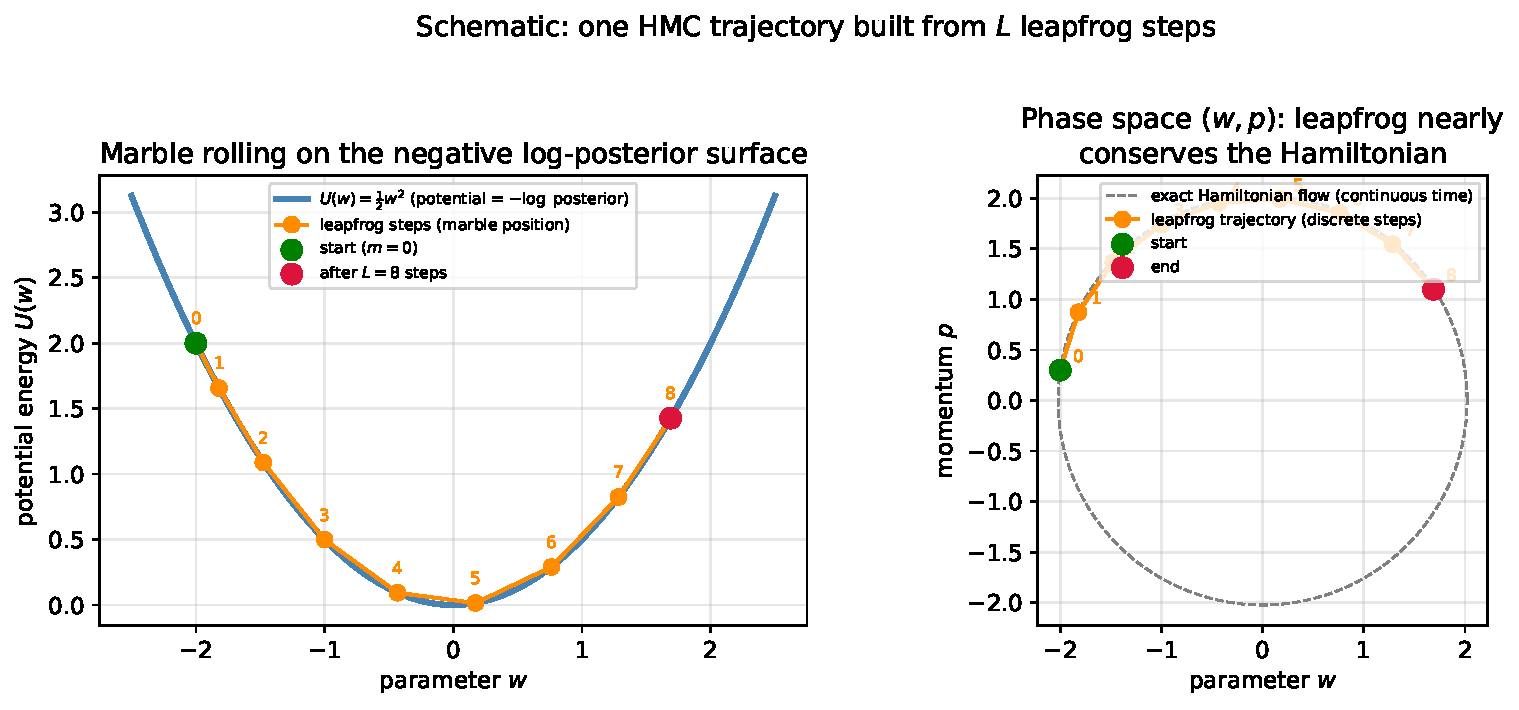
\includegraphics[width=0.95\textwidth]{fig_leapfrog_schematic.pdf}
  \end{center}
  \textbf{Left:} the marble (orange dots, numbered by leapfrog step) rolls
  down and back up the potential well $U(w)=\tfrac12 w^2$. \textbf{Right:}
  in phase space $(w,p)$, the exact continuous-time orbit is a perfect
  ellipse (dashed grey); the discrete leapfrog steps (orange) stay very
  close to it -- this is exactly why the acceptance probability stays near 1.
\end{frame}

\begin{frame}[fragile]{Python: HMC on the Toy SABR Posterior}
  Applying HMC to the same toy $(\alpha,\rho)$ inference problem as MALA,
  using a diagonal mass matrix (to handle $\alpha$ and $\rho$ living on very
  different natural scales -- $\alpha\!\sim\!0.01$ vs.\ $\rho\!\sim\!1$):
\begin{lstlisting}
def leapfrog(w, p, eps, L, precond):
    grad = grad_log_posterior(w)
    for _ in range(L):
        p = p + 0.5*eps*grad
        w = w + eps*precond*p
        grad = grad_log_posterior(w)
        p = p + 0.5*eps*grad
    return w, p

def hmc_step(theta, eps, L, precond, mass, rng):
    p0 = rng.standard_normal(2) * np.sqrt(mass)
    w, p = leapfrog(theta.copy(), p0.copy(), eps, L, precond)
    H0 = -log_posterior(theta) + 0.5*np.sum(p0**2*precond)
    H1 = -log_posterior(w)     + 0.5*np.sum(p**2 *precond)
    accept = np.log(rng.uniform()) < (H0 - H1)
    return (w if accept else theta), accept

# Book's setting: L = 25 leapfrog steps; step size tuned via dual averaging
# to target an 80% acceptance rate (we mirror L=25 in our toy demo below).
\end{lstlisting}
\end{frame}

\begin{frame}{Toy HMC Results}
  \textbf{Illustrative only.} Running HMC with $L=25$ leapfrog steps for
  1500 iterations (300 burn-in) gives an acceptance rate of about
  \textbf{96\%} and again recovers both true parameters:
  \begin{center}
    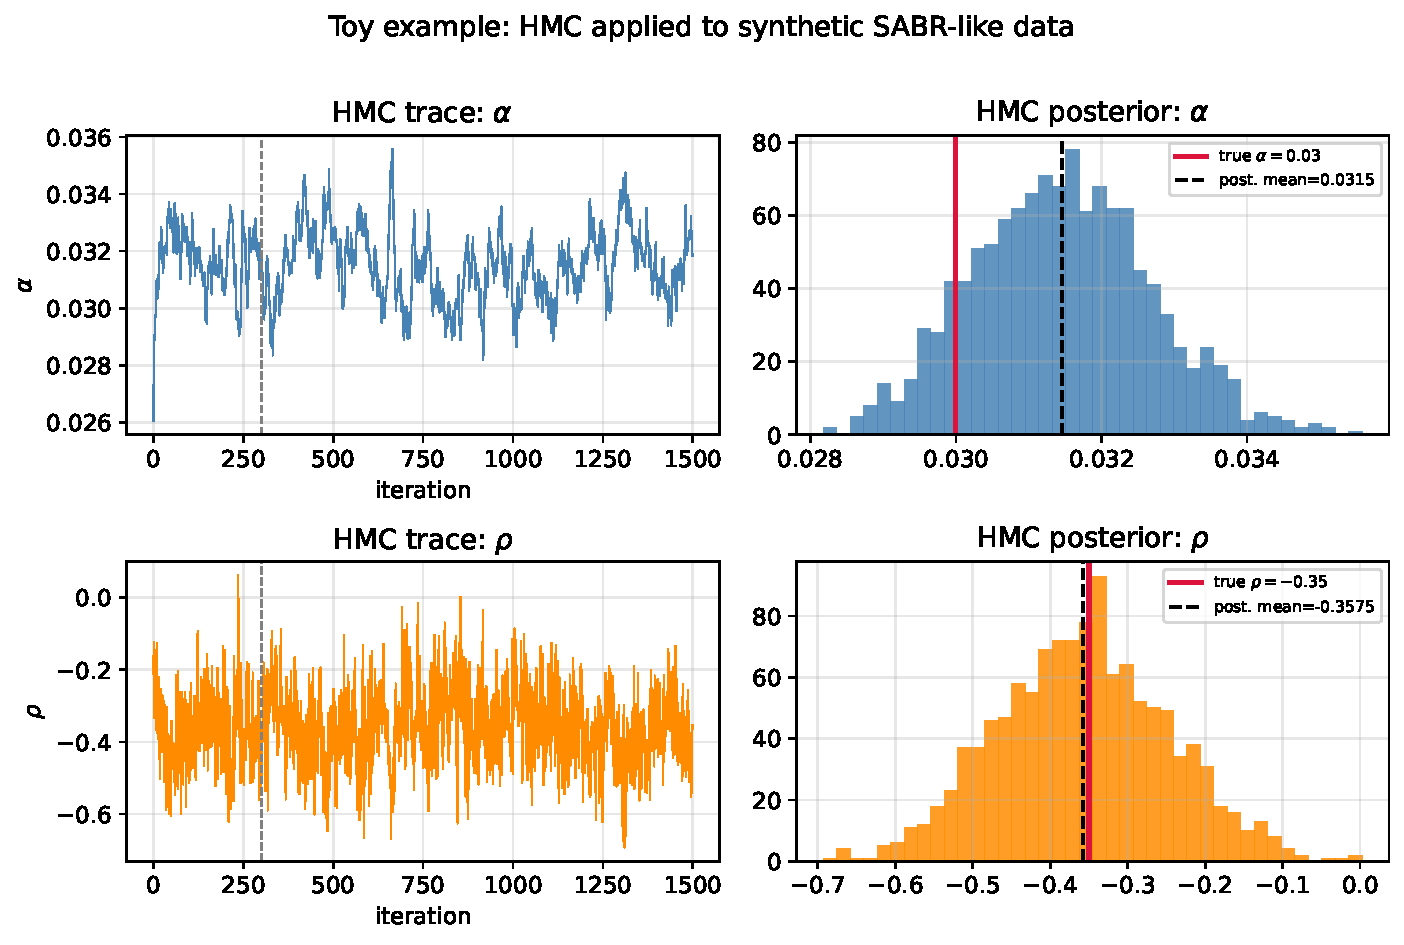
\includegraphics[width=0.85\textwidth]{fig_hmc_toy.pdf}
  \end{center}
\end{frame}

\begin{frame}{MALA vs.\ HMC: Why HMC Mixes Faster}
  Comparing the autocorrelation of the $\alpha$ chain from our toy MALA and
  HMC runs makes the payoff of ``rolling like a marble'' concrete:
  \begin{center}
    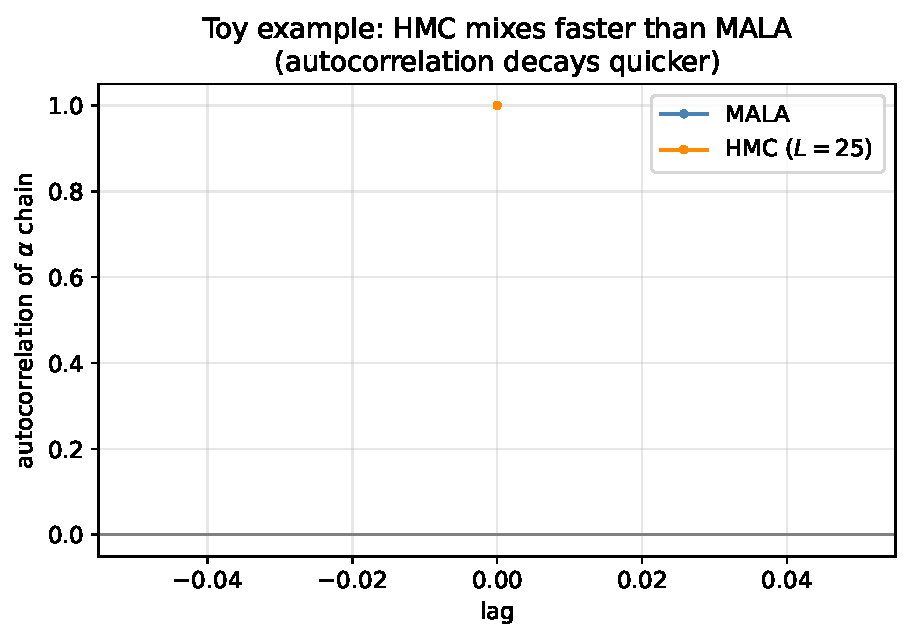
\includegraphics[width=0.62\textwidth]{fig_mala_vs_hmc_autocorr.pdf}
  \end{center}
  With $L=25$ leapfrog steps per proposal, HMC's samples decorrelate almost
  immediately, while MALA's small local nudges leave noticeable correlation
  out to lag $\sim$20. Fewer correlated samples means more \emph{effective}
  samples per iteration -- the practical payoff of HMC's physics-based
  proposals.
\end{frame}

\subsection{3.3.3 Separable Shadow Hamiltonian Hybrid Monte Carlo (S2HMC)}

\begin{frame}{S2HMC: Intuition}
  \textbf{The remaining problem with HMC.} Even HMC still produces
  autocorrelated samples. Why? The leapfrog integrator only conserves the
  \emph{true} Hamiltonian up to second order, $\mathcal{O}(\epsilon^2)$. Over
  $L$ steps this error accumulates, so $\delta H = H(\bw_{m-1},\bp_{m-1}) -
  H(\bw_m,\bp_m)$ can become large -- causing more rejections in the
  Metropolis step.

  \vspace{2mm}
  \textbf{Two obvious fixes} -- use a higher-order (more accurate)
  integrator, or shrink $\epsilon$ and $L$ -- both cost more compute time.

  \vspace{2mm}
  \textbf{A cleverer fix.} Run a backward error analysis on the leapfrog
  integrator to find a \emph{modified} (``shadow'') Hamiltonian that the
  leapfrog integrator conserves \emph{almost exactly} -- much better than it
  conserves the true Hamiltonian. Sample using the shadow Hamiltonian
  instead, then correct for the (small) difference so we still target the
  true posterior.
\end{frame}

\begin{frame}{The Shadow Hamiltonian Expansion}
  \begin{block}{Shadow Hamiltonian as an asymptotic expansion (Eq.~3.21--3.22)}
  \begin{align}
    \tilde{\Ham} &= \Ham + \epsilon \Ham_2 + \epsilon^2 \Ham_3 + \epsilon^3 \Ham_4 + \ldots \\
    \tilde{\Ham}^{[k]} &= \Ham + \epsilon \Ham_2 + \epsilon^2 \Ham_3 + \epsilon^3 \Ham_4 + \ldots = \tilde{\Ham} + \mathcal{O}(\epsilon^k)
  \end{align}
  \end{block}
  \textbf{Symbols:} $\tilde{\Ham}$ -- the (infinite-series) shadow
  Hamiltonian; $\tilde{\Ham}^{[k]}$ -- a $k$-th order truncation used in
  practice to keep the expansion from diverging. By comparing Taylor
  coefficients between the true flow and the leapfrog-generated flow, the
  correction terms $\Ham_k$ can be derived explicitly. For symplectic
  (structure-preserving) integrators like leapfrog, these modified equations
  can themselves be treated as Hamiltonian.
\end{frame}

\begin{frame}{Fourth-Order Shadow Hamiltonian}
  This chapter uses a \textbf{fourth-order truncation} $\tilde\Ham^{[4]}$,
  which is conserved with accuracy $\mathcal{O}(\epsilon^4)$ by the leapfrog
  integrator -- two orders better than the true Hamiltonian's
  $\mathcal{O}(\epsilon^2)$.
  \begin{block}{Fourth-order shadow Hamiltonian (Eq.~3.23)}
  \begin{equation}
    \tilde{\Ham}^{[4]} = U(\bw) + K(\bp) + \frac{\epsilon^2}{12}\mathrm{K}_\bp^T \mathrm{U}_{\bw\bw}\mathrm{K}_\bp - \frac{\epsilon^2}{24}\mathrm{U}_\bw^T \mathrm{K}_{\bp\bp}\mathrm{U}_\bw + \mathcal{O}(\epsilon^4)
  \end{equation}
  \end{block}
  \textbf{Symbols:} $\mathrm{U}_\bw$, $\mathrm{K}_\bp$ -- Jacobians (gradients)
  of the potential/kinetic energy; $\mathrm{U}_{\bw\bw}$, $\mathrm{K}_{\bp\bp}$
  -- their Hessians.

  \vspace{2mm}
  \textbf{Problem:} this $\tilde\Ham^{[4]}$ mixes $\bw$ and $\bp$ together
  (it is \emph{non-separable}) -- expensive to work with, requiring tuning
  of extra momentum-acceptance criteria.
\end{frame}

\begin{frame}{Making It Separable: S2HMC}
  \textbf{The fix (Sweet et al., 2009).} Pre-process the parameter and
  momentum vectors, \emph{before} running the ordinary leapfrog integrator,
  so that the resulting shadow Hamiltonian becomes \textbf{separable} again
  (a clean sum of a potential term and a kinetic term).
  \begin{block}{Separable shadow Hamiltonian (Eq.~3.24)}
  \begin{equation}
    \tilde{\Ham}(\bw,\bp) = U(\bw) + K(\bp) + \frac{\epsilon^2}{24}\mathrm{U}_\bw^T \mathbf{M}^{-1} \mathrm{U}_\bw + \mathcal{O}(\epsilon^4)
  \end{equation}
  \end{block}
  Positions and momenta are propagated on this shadow Hamiltonian after a
  \textbf{reversible mapping} $(\hat\bw,\hat\bp) = \mathcal{X}(\bw,\bp)$,
  found via fixed-point iteration:
  \begin{block}{Reversible mapping (Eq.~3.25--3.26)}
  \begin{align}
    \hat\bp &= \bp - \frac{\epsilon}{24}\Big[\mathrm{U}_\bw(\bw+\epsilon\mathbf{M}^{-1}\hat\bp) - \mathrm{U}_\bw(\bw-\epsilon\mathbf{M}^{-1}\hat\bp)\Big] \\
    \hat\bw &= \bw + \frac{\epsilon^2\mathbf{M}^{-1}}{24}\Big[\mathrm{U}_\bw(\bw+\epsilon\mathbf{M}^{-1}\hat\bp) + \mathrm{U}_\bw(\bw-\epsilon\mathbf{M}^{-1}\hat\bp)\Big]
  \end{align}
  \end{block}
\end{frame}

\begin{frame}{S2HMC: Post-Processing and Importance Weights}
  After leapfrog is run on $(\hat\bw,\hat\bp)$, the mapping is
  \textbf{reversed} using another fixed-point iteration:
  \begin{block}{Reverse mapping (Eq.~3.27--3.28)}
  \begin{align}
    \bw &= \hat\bw - \frac{\epsilon^2\mathbf{M}^{-1}}{24}\Big[\mathrm{U}_\bw(\bw+\epsilon\mathbf{M}^{-1}\hat\bp) + \mathrm{U}_\bw(\bw-\epsilon\mathbf{M}^{-1}\hat\bp)\Big] \\
    \bp &= \hat\bp + \frac{\epsilon}{24}\Big[\mathrm{U}_\bw(\bw+\epsilon\mathbf{M}^{-1}\hat\bp) - \mathrm{U}_\bw(\bw-\epsilon\mathbf{M}^{-1}\hat\bp)\Big]
  \end{align}
  \end{block}
  \textbf{Importance weights.} Because we actually sampled from the shadow
  density (not the true one), \emph{importance weights} are computed after
  sampling -- based on the difference between the true and shadow
  Hamiltonians -- to correct back to the true target posterior.

  \vspace{2mm}
  \textbf{Neat fact:} S2HMC \emph{degenerates exactly to HMC} when the shadow
  Hamiltonian is set equal to the true Hamiltonian -- so S2HMC is again a
  strict generalisation, this time of HMC.
\end{frame}

\begin{frame}[fragile]{Python: Sketch of the S2HMC Reversible Mapping}
  This is a structural sketch of the fixed-point solve in
  Eqs.~3.25--3.26 (illustrative -- not a full production implementation):
\begin{lstlisting}
def s2hmc_forward_map(w, p, eps, Minv, grad_U, n_fp=6):
    """Fixed-point iteration for the reversible mapping (w,p) -> (what, phat)."""
    what, phat = w.copy(), p.copy()
    for _ in range(n_fp):                      # iterate to convergence
        gplus  = grad_U(w + eps*Minv*phat)
        gminus = grad_U(w - eps*Minv*phat)
        phat = p - (eps/24.0) * (gplus - gminus)
        what = w + (eps**2 * Minv/24.0) * (gplus + gminus)
    return what, phat

# Usage inside one S2HMC iteration:
#   1. what, phat = s2hmc_forward_map(w, p, eps, Minv, grad_U)
#   2. what, phat = leapfrog(what, phat, eps, L, Minv)      # ordinary leapfrog
#   3. w, p       = s2hmc_reverse_map(what, phat, eps, Minv, grad_U)
#   4. accept/reject using the SHADOW Hamiltonian, then reweight samples
#      by the true/shadow density ratio (importance weights).
\end{lstlisting}
\end{frame}

\begin{frame}{Comparing MALA, HMC and S2HMC}
  \begin{table}[]
    \small
    \centering
    \begin{tabular}{lccc}
      \toprule
      & MALA & HMC & S2HMC \\
      \midrule
      Uses gradient info? & Yes (1st order) & Yes & Yes \\
      Simulated dynamics & Langevin (1 step) & Hamiltonian, $L$ steps & Hamiltonian, $L$ steps \\
      Integrator & Euler-Maruyama & Leapfrog & Pre/post-processed leapfrog \\
      Energy conserved to & -- & $\mathcal{O}(\epsilon^2)$ & $\mathcal{O}(\epsilon^4)$ \\
      Extra correction & MH accept/reject & MH accept/reject & MH accept/reject + \\
      & & & \quad importance weights \\
      Special case of & -- & MALA when $L=1$ & HMC when shadow $=$ true $\Ham$ \\
      \bottomrule
    \end{tabular}
  \end{table}
  \textbf{Book's finding (previewed):} S2HMC tends to allow larger, more
  efficient steps (fewer rejections) at the cost of somewhat higher posterior
  standard deviations in this chapter's experiments -- more in Section 3.5.
\end{frame}

% =================================================================
\section{3.4 Numerical Experiments}
% =================================================================

\subsection{3.4.1 Data Description}

\begin{frame}{Data Used in This Chapter}
  Two datasets are used to calibrate and compare MALA, HMC and S2HMC:
  \begin{itemize}
    \item \textbf{Simulated data:} generated directly from the SABR model
      with known true parameters
      $\{\alpha=0.0130,\ \rho=-0.23,\ \nu=1.21\}$
      for the \textbf{1W into 1Y} swaption. Because the truth is known here,
      this dataset checks whether each MCMC method can \emph{recover} the
      correct parameters.
    \item \textbf{Real-world data:} South African Rand (ZAR) swaption market
      data, for the \textbf{6M into 1Y} swaption, as observed on
      \textbf{28 June 2024}, extracted from a calibrated model from a market
      data provider.
  \end{itemize}
  \vspace{2mm}
  Using both lets the chapter validate correctness (simulated data, known
  truth) and real-world applicability (ZAR market data) side by side.
\end{frame}

\subsection{3.4.2 Performance Metrics}

\begin{frame}{Performance Metrics Used}
  Predictive performance on \textbf{unseen} data is assessed using four
  standard regression metrics:
  \begin{block}{Metrics}
  \begin{align*}
    \text{MSE} &= \frac{1}{n}\sum_i (y_i - \hat y_i)^2 &
    \text{MAE} &= \frac{1}{n}\sum_i |y_i - \hat y_i| \\
    \text{MAPE} &= \frac{1}{n}\sum_i \left|\frac{y_i - \hat y_i}{y_i}\right| &
    R^2 &= 1 - \frac{\sum_i (y_i-\hat y_i)^2}{\sum_i (y_i - \bar y)^2}
  \end{align*}
  \end{block}
  where $y_i$ is the observed volatility, $\hat y_i$ the model-predicted
  volatility, and $\bar y$ the sample mean.

  \vspace{2mm}
  \textbf{Experimental setup (as reported):} five chains of 2000 samples per
  method, with a burn-in of 1000; $\mathbf{M}=\mathbf{I}$ throughout; 25
  leapfrog/integration steps for HMC and S2HMC; step sizes tuned via dual
  averaging targeting a 60\% acceptance rate for MALA and 80\% for HMC/S2HMC.
\end{frame}

% =================================================================
\section{3.5 Results and Discussions}
% =================================================================

\begin{frame}{Calibration on Simulated Data (Table 3.1)}
  \small
  The book reports that MALA, HMC$_{25}$ and S2HMC$_{25}$ all reproduce the
  parameters that generated the simulated 1W into 1Y swaption data closely:
  \begin{table}[]
    \centering
    \begin{tabular}{lcccc}
      \toprule
      Parameter & True & MALA & HMC$_{25}$ & S2HMC$_{25}$ \\
      \midrule
      $\alpha$ & 0.0130 & 0.0129 (0.0191) & 0.0129 (0.0264) & 0.0130 (0.0277) \\
      $\rho$   & $-0.23$ & $-0.2301$ (0.0092) & $-0.2302$ (0.0106) & $-0.2303$ (0.0104) \\
      $\nu$    & 1.21 & 1.2147 (0.0098) & 1.2116 (0.0131) & 1.2106 (0.0136) \\
      \bottomrule
    \end{tabular}
  \end{table}
  \footnotesize (Values in parentheses are posterior standard deviations.)

  \vspace{2mm}
  \normalsize \textbf{The book reports} that \textbf{S2HMC produces the
  highest standard deviations} for each parameter, while \textbf{MALA has the
  lowest} -- i.e.\ MALA's posterior looks the most confident, though (as we
  saw with autocorrelation) it explores less efficiently per iteration.
\end{frame}

\begin{frame}{Calibration on ZAR Market Data (Table 3.2)}
  \small
  Results for the real 6M into 1Y ZAR swaption data (28 June 2024):
  \begin{table}[]
    \centering
    \begin{tabular}{lccc}
      \toprule
      Parameter & MALA & HMC$_{25}$ & S2HMC$_{25}$ \\
      \midrule
      $\alpha$ & 0.0347 (0.0027) & 0.0347 (0.0029) & 0.0347 (0.0031) \\
      $\rho$   & 0.6004 (0.0043) & 0.6001 (0.0044) & 0.6004 (0.0045) \\
      $\nu$    & 0.9176 (0.0044) & 0.9182 (0.0051) & 0.9183 (0.0053) \\
      \bottomrule
    \end{tabular}
  \end{table}
  \normalsize \textbf{The book reports} that all three methods \textbf{agree
  closely} on the calibrated parameters, and again \textbf{S2HMC produces the
  largest standard deviations while MALA produces the lowest} -- consistent
  with the simulated-data findings, suggesting this is a general pattern
  rather than a coincidence of one dataset.
\end{frame}

\begin{frame}{Predictive Performance on Unseen Data (Tables 3.3--3.4)}
  \small
  \textbf{Simulated 1W into 1Y (unseen) data:}
  \begin{table}[]
    \centering
    \begin{tabular}{lccc}
      \toprule
      Metric & MALA & HMC$_{25}$ & S2HMC$_{25}$ \\
      \midrule
      $R^2$   & 0.9999992851 & 0.999999230 & 0.999999659 \\
      MSE     & 0.0007668415 & 0.000825566 & \textbf{0.000365645} \\
      MAPE    & 0.0004271379 & 0.00046407  & \textbf{0.0003041687} \\
      MAE     & 0.0220524944 & 0.023652592 & \textbf{0.015996114} \\
      \bottomrule
    \end{tabular}
  \end{table}
  \textbf{ZAR 6M into 1Y (unseen) market data:}
  \begin{table}[]
    \centering
    \begin{tabular}{lccc}
      \toprule
      Metric & MALA & HMC$_{25}$ & S2HMC$_{25}$ \\
      \midrule
      $R^2$   & 0.9999933461 & 0.9999932867 & \textbf{0.9999934771} \\
      MSE     & 0.0124373011 & 0.0125490858 & \textbf{0.0121925901} \\
      MAPE    & 0.0007746001 & \textbf{0.0007267914} & 0.0007388930 \\
      MAE     & 0.0882670898 & \textbf{0.0854889729} & 0.0856298624 \\
      \bottomrule
    \end{tabular}
  \end{table}
  \normalsize \textbf{The book reports} that all methods perform similarly on
  unseen data, with \textbf{HMC and S2HMC displaying the best performance}
  across the various metrics.
\end{frame}

\begin{frame}{Qualitative Findings: Fitting the Skew}
  \textbf{The book reports:}
  \begin{itemize}
    \item On the \textbf{simulated} 1W into 1Y skew, all three methods fit
      the data well, with predictions \textbf{most confident near the
      at-the-money (ATM) point} and progressively less confident towards the
      wings of the skew -- and \textbf{less confident on the right wing than
      the left wing}.
    \item On the \textbf{ZAR market-observed} 6M into 1Y skew, the same
      general pattern holds, except the methods are confident in their
      predictions on the \textbf{left wing} specifically.
    \item Negative log-likelihood convergence traces (tracked across
      samples) show that \textbf{all three methods converge} on both the
      simulated and ZAR market-observed data.
  \end{itemize}
  \vspace{2mm}
  \textbf{Intuition:} confidence bands are narrow where there is the most
  ``pull'' from data (near the liquid ATM point) and widen out where the
  model is extrapolating further from where $\alpha$ is best identified.
\end{frame}

\begin{frame}{Qualitative Findings: Posterior Shapes}
  \textbf{The book reports} that, on both the simulated and ZAR
  market-observed swaption data, the three MCMC approaches \textbf{agree on
  the shape} of the marginal posterior distributions for $\alpha$, $\rho$
  and $\nu$.

  \vspace{2mm}
  \textbf{Why this matters in practice:}
  \begin{itemize}
    \item Practitioners can use these posterior distributions to understand
      the \emph{range} of plausible parameter values, not just a single
      point estimate -- something conventional calibration techniques (like
      maximum-likelihood fitting) do not directly provide.
    \item This makes it easier to construct realistic \textbf{stress
      scenarios} for the SABR parameters, relevant for e.g.\ economic capital
      calculations that depend on how the volatility skew could move.
  \end{itemize}
\end{frame}

% =================================================================
\section{3.6 Conclusions}
% =================================================================

\begin{frame}{Chapter Summary}
  \begin{itemize}
    \item Fitting the volatility skew matters for practitioners trading
      non-linear interest-rate derivatives, and \textbf{SABR} is the standard
      model used in that market.
    \item This chapter presented a (book-reported) \textbf{first-in-literature
      probabilistic framework} to infer the volatility skew in interest-rate
      markets using SABR, calibrated on both simulated and ZAR-observed
      swaption data.
    \item Three MCMC samplers were built up from first principles:
      \textbf{MALA} (gradient-nudged random walk),
      \textbf{HMC} (physics-based, momentum + leapfrog),
      and \textbf{S2HMC} (shadow-Hamiltonian refinement of HMC).
    \item \textbf{The book reports:} all three methods reproduce the observed
      skew on both datasets and perform similarly on unseen data, with
      \textbf{S2HMC showing marginal outperformance}. Confidence bands are
      tightest near the at-the-money point and widen towards the wings.
  \end{itemize}
\end{frame}

\begin{frame}{Limitations and What's Next}
  \textbf{The book notes} this work could be extended by:
  \begin{itemize}
    \item Considering the \textbf{entire} interest-rate volatility surface,
      rather than just the single 1W into 1Y and 6M into 1Y swaption slices
      used here.
    \item Comparing SABR against \textbf{other models} that can also capture
      the volatility skew.
  \end{itemize}

  \vspace{3mm}
  \textbf{Looking ahead:} the next chapter turns to learning the
  \emph{entire} volatility surface using \textbf{sparse Gaussian process
  models}, applied to developed and emerging equity option markets --
  building directly on the Bayesian/MCMC machinery established here.
\end{frame}

\begin{frame}{Key Takeaways}
  \begin{enumerate}
    \item \textbf{SABR} models volatility itself as a random process,
      correlated with the asset price -- fixing the shortcomings of constant-
      and local-volatility models for capturing the smile/skew.
    \item \textbf{MH $\to$ MALA $\to$ HMC $\to$ S2HMC} form a natural
      progression: each adds a smarter way of proposing the next MCMC state,
      trading extra computation for faster mixing and lower autocorrelation.
    \item \textbf{HMC's core trick} is treating sampling as physics: momentum
      plus a (nearly) energy-conserving leapfrog integrator lets proposals
      travel far while staying likely to be accepted.
    \item \textbf{S2HMC} squeezes out further efficiency by having the
      integrator conserve a modified (\emph{shadow}) Hamiltonian almost
      exactly, correcting back to the true posterior via importance weights.
    \item These same MCMC building blocks reappear throughout the rest of
      this book -- make sure they are solid before moving on.
  \end{enumerate}
\end{frame}

\end{document}
